\chapter{REVISÃO DA LITERATURA}
\thispagestyle{empty}

\section{Projetos}

\citeonline[p. 8]{meredith2011project} definem que projetos tratam da realização de são tarefas específicas e finitas, de grande ou pequena escala, com um prazo de execução e um orçamento estipulado. \citeonline{turner2014handbook}, por sua vez, dispõe que projetos são tarefas com uma data final, onde caso esta data não implique na entrega do projeto, estabelecerá uma entrega do produto presente, com a criação de outro projeto para entregar as tarefas restantes.

Para \citeonline{kerzner2013project} um projeto pode ser caracterizado por uma serie de atividades e tarefas realizadas com um objetivo especifico para ser completado sob certas especificações. Projetos também devem definir datas, de inicio e fim; limites de recursos e custos; bem como o quantitativo de pessoas e equipamentos que envolverá.

Assim, pode-se compreender que todo projeto é essencialmente temporário e único, ou ainda, finito e regular, e deve visar o desenvolvimento de um novo produto ou serviço. Portanto, espera-se que toda gestão de projetos possa, igualmente, fornercer caracteristicas próprias para uma competência adequada.

\section{Gestão de Projetos}

Por definição, de acordo com \citeonline{pmiguide2001}, a gestão de projetos implica no uso de ferramentas, técnicas, e ainda na competência de utilizar o conhecimento de conceitos; caracteristicas próprias e particulares; bem como fatores críticos de sucesso para o aprimoramento e entrega de projetos de excelência.

Para \citeonline[p. 74]{kerzner2013project} a GP pode também ser considerada uma metodologia que consiste em um processo repetitivo usado em projetos com o objetivo de alcançar sua maturidade. Afirma-se ainda que qualquer metodologia, inclusive a mais simples, pode representar um caso de sucesso como prática de GP se for bem aceita na organização em questão. Entretanto, ao utilizar uma metodologia de GP de sucesso, a probabilidade de que a organização seja bem aceita como entregadora de bons projetos será elevada\cite{kerzner2013project}.

Alguns autores, a garantia de que os objetivos definidos de projeto serão alcançados depende de um processo disciplinado, por parte da GP, que respeite custos, prazos e desempenho requeridos e que ocorra através do envolvimento de pessoas em atividades de planejamento e controle numa organização \cite{dinsmore2009ama, meredith2011project}.

\section{Gestão de Programas}

Programas podem ser entendidos por estruturas que consistem em uma equipe principal e um conjunto de equipes de projeto que averiguam capacidade de decisão e autoridade de um membro definitivo, isto é, um gerente de programa que assegura a direção e as decisões desta estrutura. Estas estruturas visam alcançar um determinado objetivo dentro de uma estratégia.\cite{brown2008handbook}.

\citeonline{Rijke20141197} avalia que apesar da dificuldade geral em distinguir um programa de um projeto, a gestão de programas deve ser considerada mais extensa que gestão de projetos, pois ela abrange áreas em que projetos singulares não se encontram. Vale ressaltar também que o gestor de programa tem hábitos mais estrategicos que podem interferir na GP \cite{lycett2004289}.

Assim, a gestão de programas tem sido cada vez mais adotada por organizações com o objetivo de implementar estratégias que integrem melhor seus projetos e ferramentas, sem permitir que o desempenho possa desonrientar a natureza estratégica das decisões.


\section{Gestão de Portfólio}

A gestão de portfólio, conhecida também por Gestão de Portfólio de Projetos (GPP)\nomenclature{GPP}{Gestão de Portfólio de Projetos}, surgiu a partir da necessidade de gerenciar investimentos em projetos nas organizações. Seu processo dinâmico e integrado visa avaliar o alinhamento estratégico e a viabilidade da execução simultânea de diversos projetos ao mesmo tempo. Esses projetos passam por uma introspecção que os seleciona e organiza de acordo com sua priorização em um portfólio \cite{meredith2011project, kerzner2013project}.

De acordo com \citeonline[p. 27]{burke2013project}, um portfólio pode abrigar conjuntos de projetos, programas e até mesmo outros portfólios que não precisam estar diretamente relacionados, mas que se reúnem por uma questão de otimização e controle. A figura \ref{port_prog_proj} demonstra sobre a relação entre portfólio, programas e projetos.

\begin{figure}[ht]
  \centering
  \scalebox{0.4}{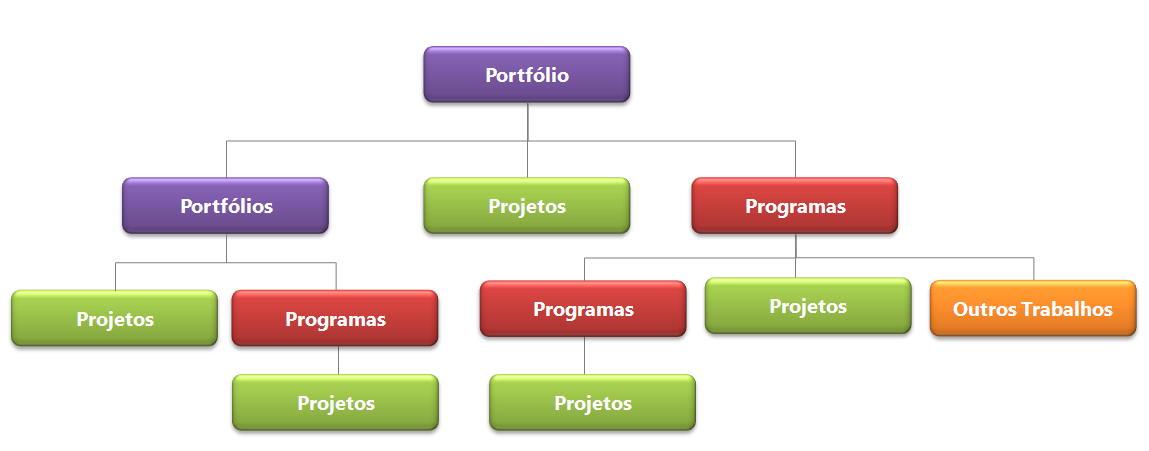
\includegraphics{figuras/port-prog-proj}}
  \caption{Relação Portfólio, Programas e Projetos. Fonte: \cite{pmi2006}}
  \label{port_prog_proj}
\end{figure}

\citeonline[p 11]{pmiguide2001} estabelece que o critério de agrupamento de um portfólio deve visar a facilitação na gestão para que seja possível atingir os objetivos estratégicos de uma organização. É definido ainda que toda gestão de portfólio fique sob responsabilidade de um escritório de gestão de projetos (\textit{Project Management Office} - PMO)\nomenclature{PMO}{Escritório de Gestão de Projetos (\textit{Project Management Office})} \nomenclature{PMI}{Instituto de Gerenciamento de Projetos (\textit{Project Management Institute})} \nomenclature{PMBOK}{\textit{Project Management Body of Knowledge}}. A figura \ref{estrategia_portfolio} representa os processos incorporados pela Gestão de Portfólio.

\begin{figure}[ht]
  \centering
  \scalebox{0.4}{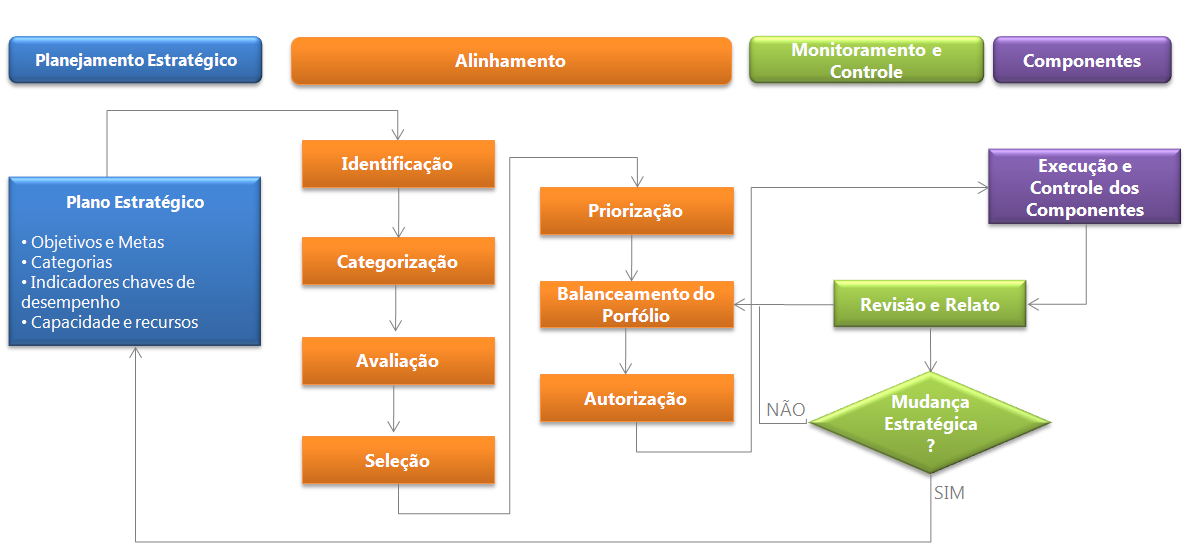
\includegraphics{figuras/estrategia-portfolio}}
  \caption{Processos de Gestão de Portfólio. Fonte: \cite{pmi2006}}
  \label{estrategia_portfolio}
\end{figure}

\section{Escritorio de Gestão de Projetos}

Para \citeonline{dinsmore2005pmo} a principal expectativa empregada por um PMO esta relacionada a suporte e orientação, ao processo de desenvolvimento e gerenciamento de projetos mais eficiente e eficaz o possível, e ao uso de metodologias e recursos de planejamento e análise de projetos padronizadas.

Assim, as responsabilidades de um PMO podem variar de acordo com a centralização empregada na organização, uma vez que esta relacionada a padronização dos processos de gestão. As ferramentas e técnicas a serem empregadas ficam sob critério do gestor responsável pelo PMO \cite{pmiguide2001}.

Através de um estudo, \citeonline{Pemsel201331} identificou três principais atividades que são esperadas do PMO:

\begin{itemize}
  \item Promover e facilitar o desenvolvimento estratégico da GP, bem como o uso estratégico de objetos que sejam empreendidos na GP;
  \item Planejar, controlar e dar suporte a GP, sempre assegurando que o conhecimento seja compartilhado no processo para melhorar sua eficiencia;
  \item Adoção estratégias de treinamento, negociação e formação para prover o desenvolvimento de competências.
\end{itemize}


\section{Gestão Tradicional de Projetos}

Ao decorrer dos anos, o uso de abordagens de GP foram disseminado como “guia de conhecimento”, e representava um conjunto de técnicas, princípios, ações e ferramentas que supostamente seriam capazes de gerenciar qualquer projeto \cite{kolltveit2007perspectives, shenhar2007reinventing}.

Inicialmente essas abordagens mantinham o foco no planejamento e controle do produto de forma engessada sem prever instabilidade e emergências, pois acreditava que era importante entregar o produto de acordo com os requisitos previamente levantados, indiferente a dissociações naturais do dia a dia \cite{winter2006directions}.

\citeonline{shenhar2007reinventing} afirmam que alguns autores investigaram sobre a correlação das práticas adotadas de acordo com o tipo de projeto descrito e das ferramentas utilizadas, e constataram que grande parte dos projetos eram geridos sem a devida diferenciação quanto a sua natureza, e com o uso de práticas genéricas denominadas “melhores práticas”.

De acordo com \citeonline{collyer2010aim} foi reconhecido pelo PMBOK que as práticas deveriam prever planos emergências que lidassem com conformidades não previstas nos requisitos, entretanto quanto a formação da ISO 21500, utilizada como padrão pela GP, nota-se que suas técnicas e ferramentas referiam-se com frequência ao modelo Cascata, quanto ao ciclo de vida do projeto apresentado por \citeonline{boehm1988spiral}.

Como explica \citeonline{almeida2012fatores}, é natural que práticas e abordagens evoluam ao longo dos tempos, como projetos passaram a ser o centro de toda e qualquer organização, entretanto, notou-se que a prática de GP se mantinha inadequada e que grande parte das falhas gerências estavam diretamente ligadas as técnicas utilizadas nestas praticas de GP.

A motivação das abordagens de GP consideradas tradicionais estava diretamente relacionada a perspectiva de que projetos eram relativamente simples, previsíveis eque seguiam de forma linear, tornando-os fáceis de detalhar e seguir ao longo do planejamento. Possibilitando assim, uma entrega eficiente dentro do prazo \cite{turner2010perspectives, boehm1988spiral, boehm2003using, cicmil2009exploring, collyer2010aim, mir2014exploring, shenhar2007reinventing, williams2005assessing}.

Ainda, uma das vantagens descritas na prática tradicional era a capacidade robusta, isto é, a defesa de que diversos projetos poderiam sempre ser gerenciados seguindo as mesmas técnicas e ferramentas, como se fossem todos na mesma natureza. Para diversos autores a robustez de planejamento é a maior desvantagem da prática tradicional, pois projetos têm se tornado cada vez mais complexo, e o para ideal de planejar linearmente não compete lidar com irregularidades dinâmicas da realizada do mercado \cite{aguanno2004101, cicmil2009exploring, chin2004agile, shenhar2007reinventing, williams2005assessing, wysocki2011effective}.

Entretanto, \citeonline{styhre2006bureaucratization} destaca que no desejo por diminuir riscos e evitar ineficiências, o foco de gerenciar criatividade e mudanças é burocratizado e acaba por ser tornar um gerenciamento de papéis e formulários, geralmente encontrados na robustez do projeto.

Outra desvantagem notada é que por focar no planejamento e controle, essas abordagens ignoram não só a natureza do projeto, como também aspectos humanos quanto a sociabilização, contextualização e tendência a mudanças \cite{winter2006directions, highsmith2009agile}.


\section{Gestão Ágil de Projetos}

Em função as desvantagens apontadas nas abordagens tradicionais de GP, somadas ao crescimento de um mercado inovador, com demandas contínuas e necessidade pela redução de custos, resultaram no advento de novas abordagens para GP \cite{aguanno2004101, amaral2011gerenciamento, williams2005assessing}.

Em 2001, a partir de uma iniciativa em conjunto conhecida por Manifesto Ágil houve a formalização das abordagens ágeis. Seu diferencial se apresentava, simplificadamente, como um conjunto de técnicas, princípios e ferramentas que melhoravam o trabalho em time, permitindo adaptação e evoluções ao longo do projeto \cite{beck2001manifesto, berggren2008rethinking, cohn2005agile, hass2007blending, highsmith2009agile, fernandez2008agile, fitsilis2008comparing, larman2003iterative, schwaber2004agile, smith2007flexible, qumer2010empirical}.

De acordo com \citeonline{cockburn2002agile} e \citeonline{schwaber2004agile} existem quatro princípios ágeis que devem sempre ser enfatizados:

\begin{enumerate}
    \item{Indivíduos e Interações são mais importantes que processos e ferramentas;}
    \item{Colaboração com as necessidades dos clientes acima de negociação de contratos;}
    \item{Produto em funcionamento vale mais que documentação abrangente;}
    \item{Responder as mudanças independente do plano a seguir.}
\end{enumerate}

Existem também práticas e ferramentas, como a concepção de visão do produto, desenvolvimento iterativo; além do uso de ferramentas visuais de planejamento do projeto e de seus artefatos \cite{augustine2005managing, boehm2004balancing, chin2004agile, highsmith2009agile}.

Ao ressaltar a importância dos itens, entretanto, os autores destacam que eles não se excluem, o ideal é que todos sejam levados em consideração, apenas seguindo a ordem de importância \cite{aguanno2004101}.

Essas abordagens podem ser apontadas por GAP, e representaram uma alternativa para problemática das mudanças constantes, alterações a curto prazo dentro do planejamento do projeto, valorização do cliente como uma fonte de interação \cite{amaral2011gerenciamento, augustine2005managing, cohn2005agile, highsmith2009agile}.

Alguns autores, enfatizam que estas abordagens têm uma relação muito estreita com a engenharia de software, levando essas abordagens a aparecerem com frequência relacionadas ao desenvolvimento de software \cite{aguanno2004101, boehm1988spiral, beck2001manifesto, williams2005assessing}.

\citeonline{stare2014agile} afirma que durante uma entrevista os autores responsáveis pelo Manifesto Ágil ressaltaram a importância das abordagens GAP como um meio de tornar o GP uma ferramenta de sucesso no atual mercado, e que apesar de serem inicialmente aplicadas em projetos de tecnologia de informação (TI), eram igualmente apropriadas a qualquer natureza de projetos, visto que o foco destas abordagens está em reconhecer e aplicar feedback com a finalidade de lidar com incertezas.

Apesar desta declaração, \citeonline{stare2014agile} contesta que nos estudos pesquisados até o ano de 2009, em sua maioria, as práticas ágeis se referiam ao uso em projetos de TI, e que neste ano, algumas pesquisas começaram a reconhecê-las em outros campos com certo receio.

Entre as metodologias ágeis mais utilizadas, as que mais se destacam na indústria são: Scrum \cite{schwaber2004agile}, Lean Software Development \cite{poppendieck2007lean}, Crystal \cite{cockburn2004crystal}, Feature Driven Development \cite{palmer2001practical}, Adaptive Software Development \cite{highsmith2001agile} e eXtreme Programming \cite{beck2000extreme}.

Considerando a crescente necessidade da indústria por inovação e pela necessidade de redução de custos, as abordagens GAP tomaram o cenário de GP devido sua habilidade de adaptação durante o ciclo de vida dos projetos, indiferente a sua natureza. Mudanças são inevitáveis e impossíveis de prever, portanto é importante lidar com elas \cite{aguanno2004101, amaral2011gerenciamento,chin2004agile, decarlo2010extreme, highsmith2009agile, leffingwell2007scaling, williams2005assessing}.

Além disso, como atrativos para utilização de práticas ágeis se destacam: a melhora na habilidade de comunicação formal e informal, bem como a colaboração externa com a aproximação dos clientes no processo de produtos \cite{aguanno2004101, cockburn2006agile, collyer2010aim, coram2005impact, decarlo2010extreme, highsmith2001agile, williams2005assessing}

Alguns autores destacam que a proximidade do time com o projeto melhora seu desempenho e a habilidade de ser auto-gerenciáveis e responsáveis em suas tarefas \cite{augustine2005managing, boehm2004balancing, highsmith2009agile}.


Vale destacar que também existiram ideias de foram herdadas das práticas tradicionais, como o ideal de que o projeto fosse iterativo, isto é, pudesse ser incrementado ao longo do processo de produção \cite{aguanno2004101, boehm1988spiral}.

Entretanto, invés de utilizar um único plano para o projeto, GAP utilizam a ideia de iteratividade ao longo de todo processo através de pequenas fases com retorno geralmente fornecido por feedback \cite{augustine2005managing, boehm2004balancing, cohn2005agile, highsmith2009agile, schwaber2004agile}.

Para \citeonline{poppendieck2007lean} o motivo pelo qual as práticas ágeis se destacaram esta diretamente relacionado a sua capacidade de entregar produtos com rapidez e qualidade, atendendo as necessidades do cliente de forma satisfatória utilizando princípios que já haviam sido citados pela metodologia Lean de produção.

 A marca de agilidade é também propiciar uma melhoria de performance a medida que o cliente colabora mais ativamente frente a demonstração do produto; além de trazer o conceito de flexibilidade e estabilidade \cite{chin2004agile}.

Para \citeonline{aguanno2004101} uma das maiores vantagens do da GAP é a redução de riscos e falhas, a partir do memento que seu escopo pode ser definido ao longo do projeto, mudanças não se tornam transtornos e portanto não são erros.

Entre outras vantagens, é importante destacar o uso de ferramentas visuais que permitem organizar ideias, deixar claros objetivos e fases, tornar processos compreensíveis e facilitar o planejamento de projetos e gestão de portfólios, reduzindo riscos burocráticos \cite{malachiasproject}.

Alguns autores discutem que é preciso que as mudanças não sejam aplicadas apenas pela inovação do mercado, mas também na forma de pensar em GP, e consequentemente na estrutura da própria organização para que haja o correto emprego dos princípios e ferramentas observados \cite{aguanno2004101, boehm2003using, chin2004agile, cockburn2006agile, decarlo2010extreme, highsmith2009agile, leffingwell2007scaling, shenhar2007reinventing}.

Finalmente é preciso questionar se as práticas e princípios previstos nas abordagens GAP realmente se aplicam ao mercado, e se ao aplicá-los será possível entregar produtos de qualidade, com melhor custo e dentro do prazo.

\section{Repensando a Gestão de Projetos}

Através de estudos, alguns autores notaram que alguns projetos procuram utilizar GAP como uma forma de fugir de ferramentas e técnicas particulares empregadas pelas abordagens tradicionais, e acreditam que estudos mais detalhados deveriam ser realizados nesses termos \cite{conforto2010evaluating, coram2005impact, leybourne2009improvisation}.

Para \citeonline{cockburn2000selecting} toda abordagem tem seus limites, por mais bem embasada que possa ser, principalmente quando se tratam de produtos e clientes. Para que um determinado produto seja entregue com sucesso, é reconhecido que é ideal o uso de uma abordagem de GP, entretanto tanto a abordagem tradicional quanto a abordagem ágil possuem vantagens e desvantagens \cite{aguanno2004101, turner2010perspectives}.

Devido o aumento da demanda de inovação o crescimento do uso das abordagens, tanto individualmente quanto mescladas, tem sido o foco de estudos empíricos que buscam adaptá-las a diferentes tipos de projetos \cite{conforto2010evaluating}.

De acordo com o estudo de \citeonline{benassi2011evaluating} existe evidencia de aspectos positivos no que diz respeito ao uso de GAP, entre elas: aumento na velocidade em que empresas alcançam inovações; cortes em custos excessivos, entre eles custos de armazenagem e desenvolvimento; diminuição do tempo de entrega do produto; reduz falhas no atendimento aos requisitos e portanto atende melhor ao desejo do cliente ao entregar produtos de qualidade em um prazo pequeno.

Entretanto, foi identificado também que a sugestão de pouca documentação em projetos é sugerida apenas para organização que possuem times pequenos e/ou bem organizados, que não detenham restrições corporativas e de procedimentos \cite{boehm2005management,lindvall2004agile}.

Alguns estudos definiram que projetos cujo o escopo é bem definido inicialmente, onde requisitos e metas possuem baixa nível de incerteza e mudança; e que podem ser desenvolvidos sem a presença frequente do cliente podem ser bem sucedidos com o uso de abordagens tradicionais, pois precisam focar apenas no planejamento e na otimização de atividades previstas \cite{boehm2003using, coram2005impact, decarlo2010extreme, fernandez2008agile, shenhar2007reinventing, wysocki2011effective}.

Consequentemente, se o projeto for realizado em grandes corporações, independente de seu tamanho em particular, seu grau de complexidade ou sua duração; não é aconselhável que sejam utilizadas apenas abordagens GAP \cite{aguanno2004101, boehm2003using, boehm2004balancing, cockburn2000selecting, highsmith2009agile}.

Para flexibilizar produtividade e satisfazer as necessidades de grandes organização, é sugerido que modelos sejam desenvolvidos, mesclando um pouco das ferramentas, técnicas e princípios de abordagens tradicionais e com GAP \cite{batra2010balancing, barlow2011overview, boehm2004balancing, conforto2010evaluating, magdaleno2012reconciling}.

Estudos recentes vêm utilizando referências teóricas e estudos empíricos para desenvolver modelos que sigam um pouco de cada abordagem \cite{batra2010balancing, barlow2011overview, lindvall2004agile}.

\citeonline{mafakheri2008project} avalia o grau de agilidade de projeto, sob seis características: dinamismo; tamanho da equipe; comunicação; capacidade de testar resultados; conhecimento e habilidades relacionados ao produto. Não foi apresentado um estudo de caso comprovando a eficiência do modelo como uma prática de GP.

\citeonline{qumer2008evaluation} desenvolveu um modelo que pode avaliar o a grau de agilidade seguido nos processos de um produto no meio empresarial baseado em quatro dimensões: escopo de método, características da agilidade, valores ágeis e o processo. Este modelo foi avaliado pelo ponto de vista apenas dos gerentes de projeto, faltando assim o uso como prática de GP.

\citeonline{ganguly2009evaluating} utiliza quatro métricas para avaliar o uso de práticas de gerenciamento de projetos: qualidade do produto; lucratividade; adaptabilidade; e custo. Neste estudo apenas os resultados foram avaliados pelos gerentes de projeto, faltando novamente um exemplo externo.

\citeonline{binder2014project} desenvolveu um modelo que utilizasse uma combinação das abordagens focando no entendimento da ISO 21500 para grandes organizações com implicações legais e financeiras. O modelo foi desenvolvido sob um estudo de caso, porém não existe referência de uso desse modelo em prática.

